% Data aggregation server:

\begin{frame}{Requirements for the data warehouse}
  \begin{itemize}
    \item Multiple experiments (TAIGA, KASCADE, etc.);
    \item Terabytes of data (of different reconstruction level) at each site;
    \item Remote access to query results as local file systems;
    \item  On-demand data transfer by requests only;
    \item  Automatic real-time updates;
    \item  No changes to existing site infrastructure, only add-ons.
  \end{itemize}
\end{frame}

\begin{frame}{Proposed solution for data aggregation}
\textbf{Main solution components}: CVMFS, PostgreSQL, TPL
    \begin{center}
        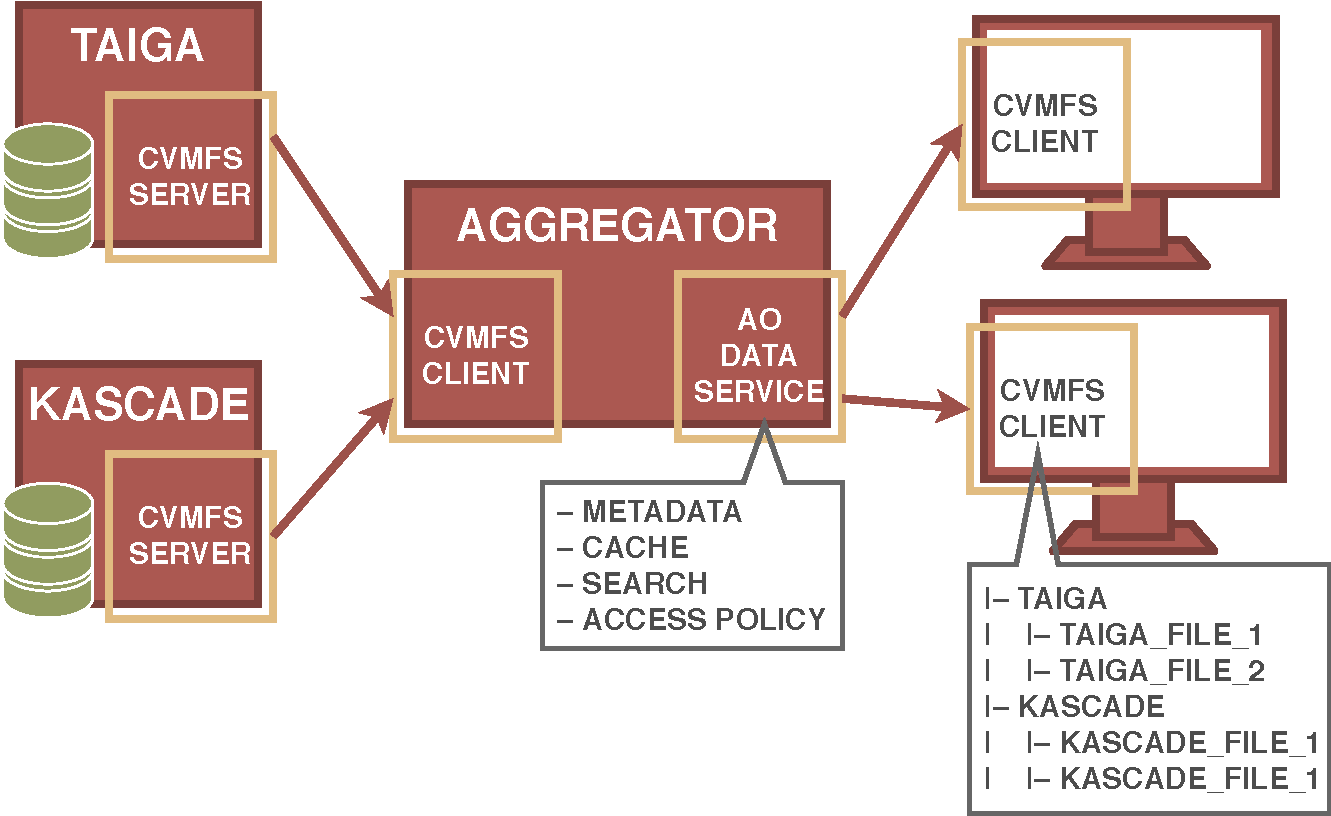
\includegraphics[width=0.82\textwidth]{pics/agr.pdf}
    \end{center}
\end{frame}


%Metadata architecture
\begin{frame}{Proposed cosmic-ray metadata structure}
    \vspace{-1.5em}
    \begin{center}
        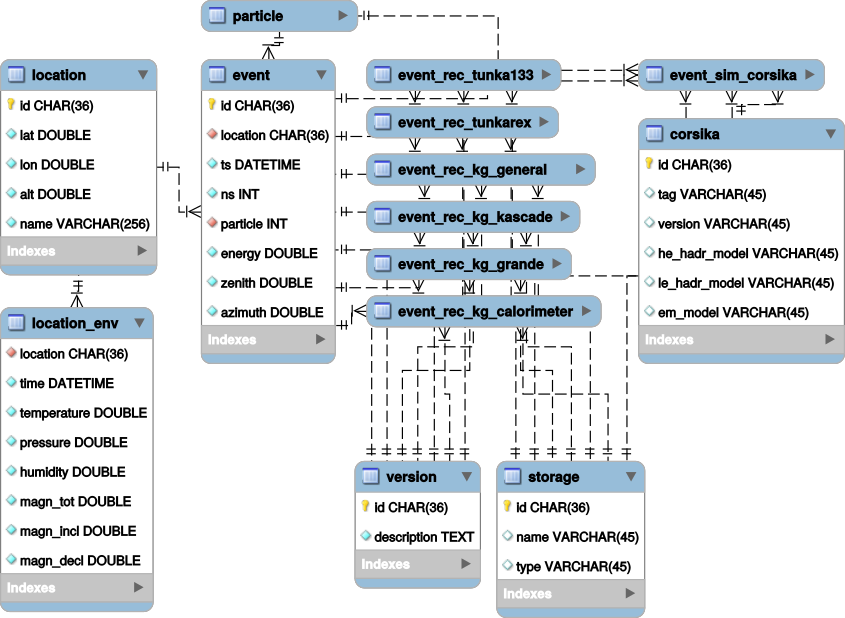
\includegraphics[width=0.82\textwidth]{pics/metadata.pdf}
    \end{center}
\end{frame}

%Data workflows
% \begin{frame}{Data workflow}
%     \vspace{-2em}
%     \centering
%     \only<1>{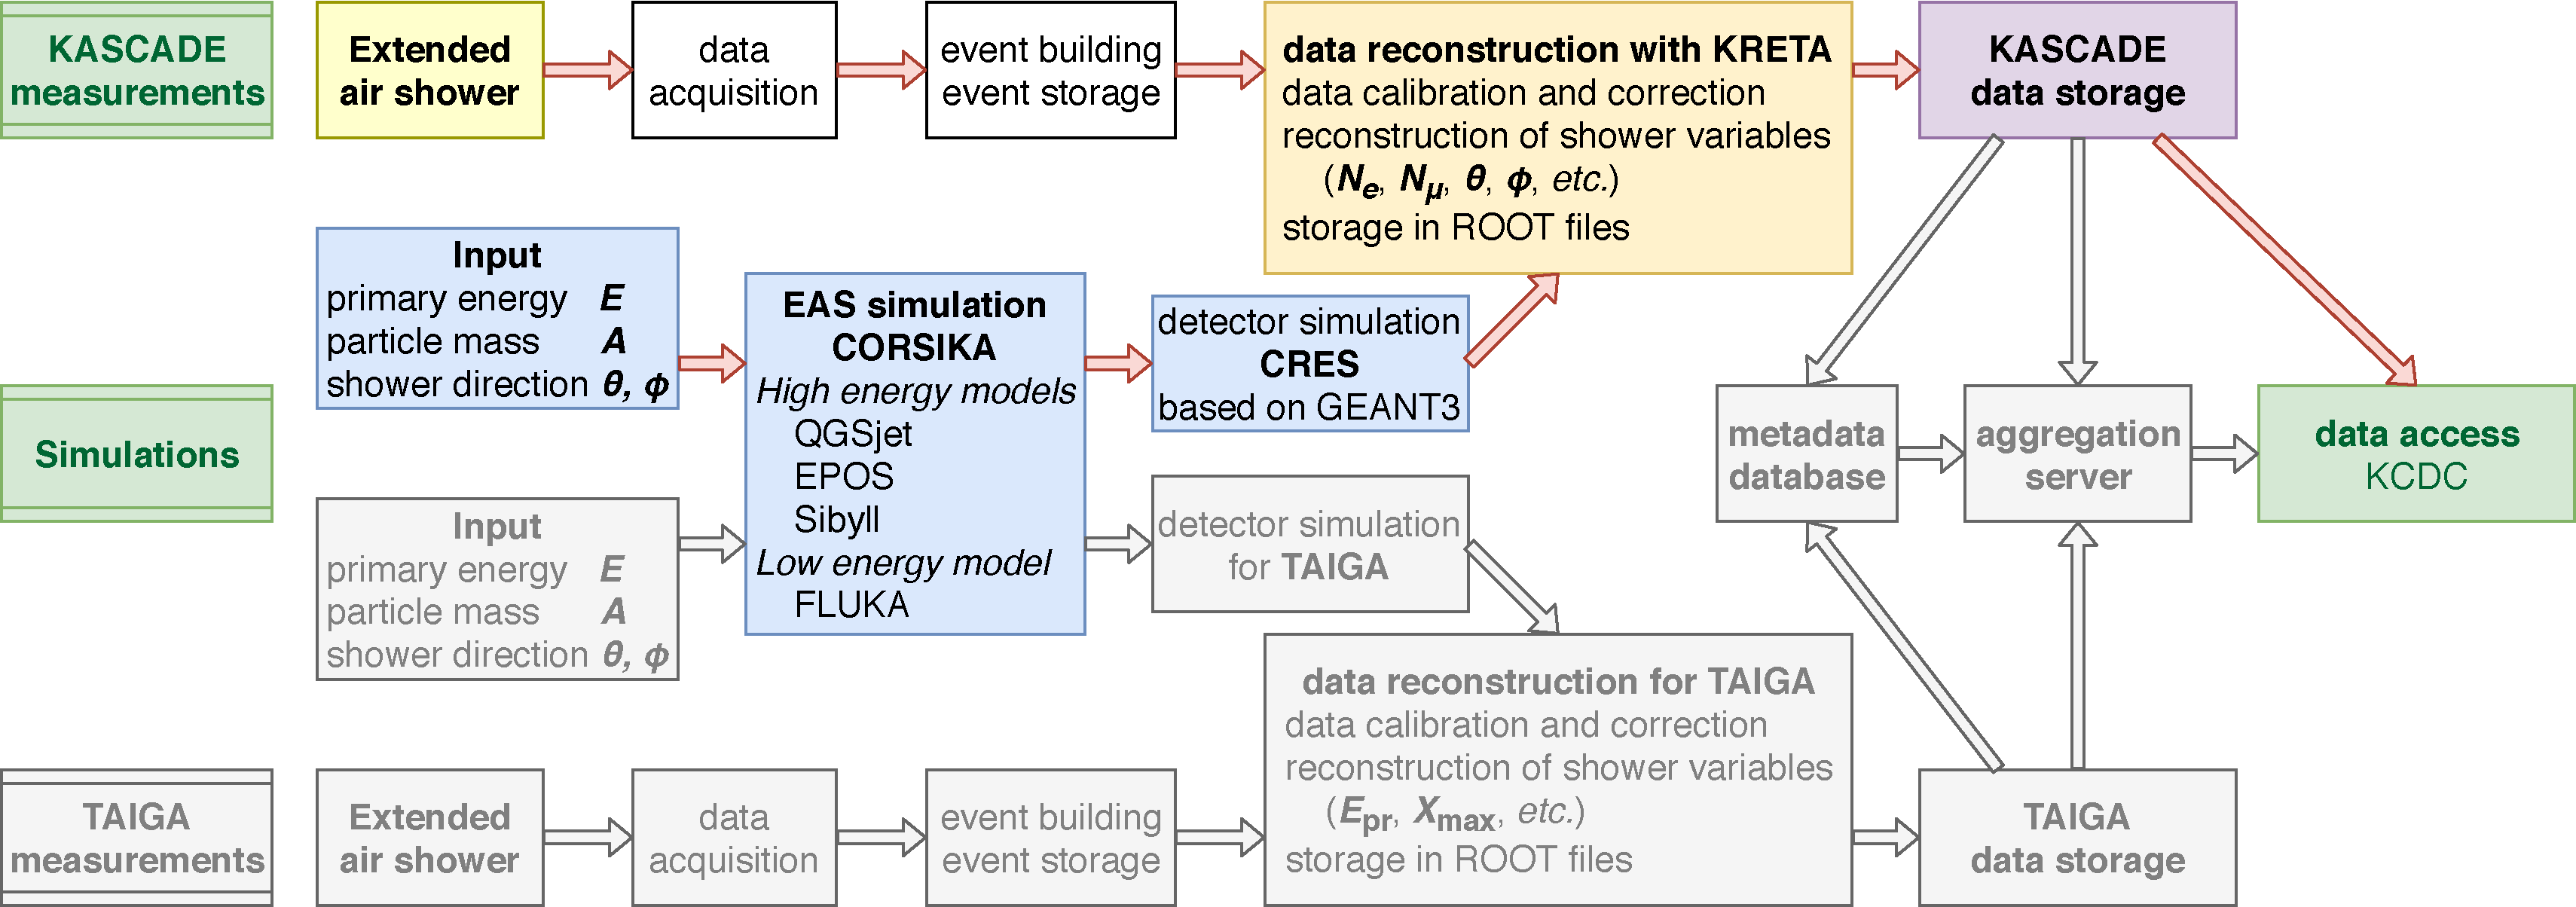
\includegraphics[width=1\textwidth]{pics/KRAD_workflow_curr.pdf}}
%     \only<2>{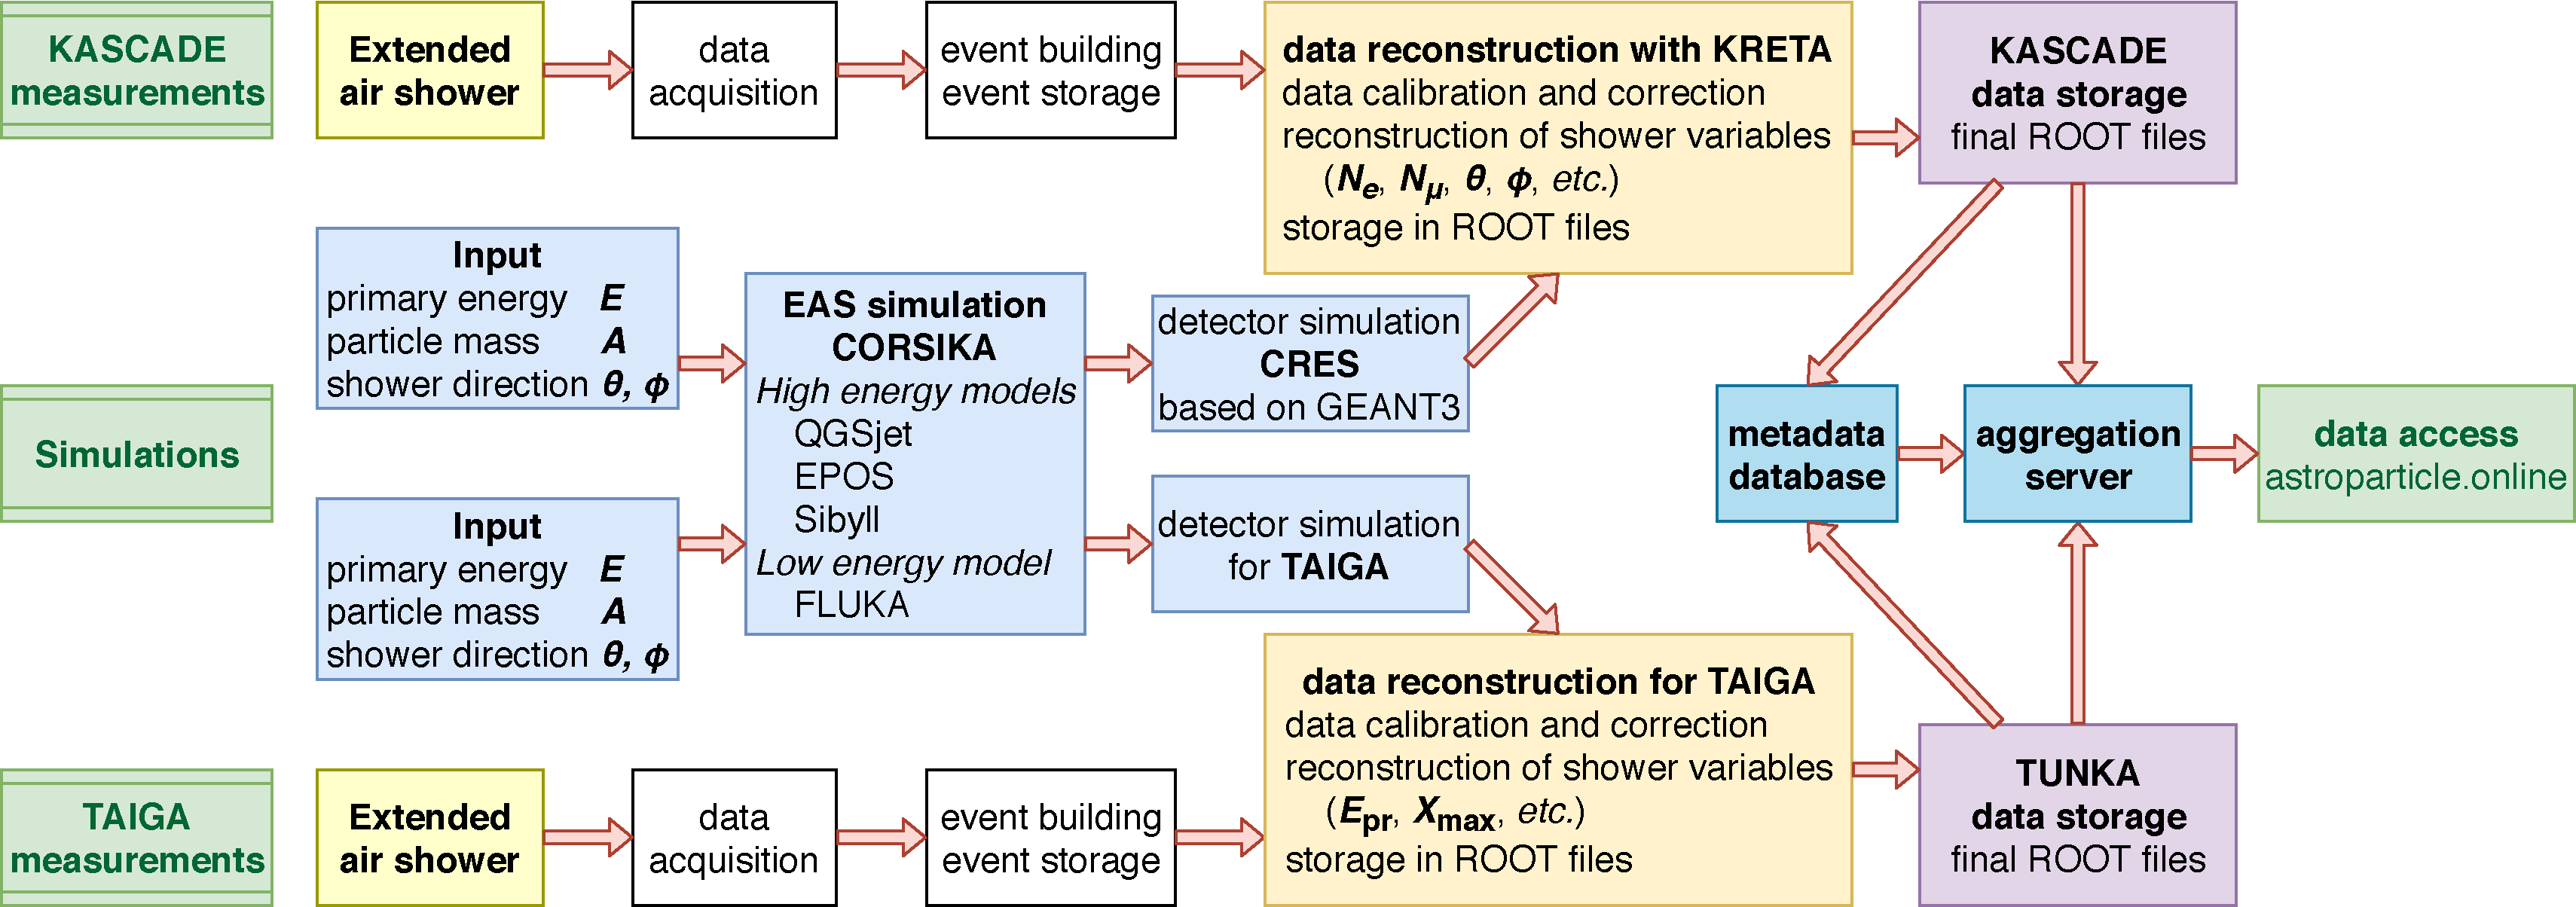
\includegraphics[width=1\textwidth]{pics/KRAD_workflow_hori.pdf}}
% \end{frame}

% TODO:
%         Data summary and challenges (no slide so far :-( )
%         Possible solutions (postgres, cvmfs, etc...)
